\lecture{9}{21 marzo 2024}
\subsection{Analisi energetica}

Consideriamo l'armonica n-esima: \(\xi _n (x,t) = A_n \sin (k_n x) \sin (\omega _n t)\). È un'onda stazionaria di modo n tra 0 e L che rispetta le opportune condizioni iniziali e che ha energia cinetica e potenziale. 
\begin{itemize}
	\item Energia cinetica: \(u_k(x,t)= \frac{1}{2} \mu \left( \frac{\partial \xi }{\partial t}  \right)^{2} = \frac{1}{2} \mu \omega _n ^{2} A_n ^{2} \sin ^{2} (k_n x) \cos ^{2} (\omega t) \), è sempre nulla sui nodi (effettivamente non si muovono su y).
	\item Energia potenziale: \(u_P (x,t)= \frac{1}{2} T \left( \frac{\partial \xi }{\partial x}  \right)^{2} = \frac{1}{2}T k_n ^{2} A_n ^{2} \cos ^{2} (k_n x) \sin  ^{2} (\omega _n t) \), è sempre nulla sui ventri.
\end{itemize}
La densità di energia meccanica si scrive quindi come:
\[
	u(x,t) = \frac{1}{2} \mu \omega _n ^{2} A_n ^{2} \sin ^{2} (k_n x) \cos ^{2} (\omega t) + \frac{1}{2}T k_n ^{2} A_n ^{2} \cos ^{2} (k_n x) \sin  ^{2} (\omega _n t)
\]
\(u(x,t)\) non è costante, nè nel tempo nè nello spazio! Inoltre si nota che \(u_P\) e \(u_K\) sono sempre sfasati di \(\pi /2\). Si può calcolare l'energia totale presente nella corda (ponendo \(m =L \mu \)):
\begin{figure}[H]
	\centering
	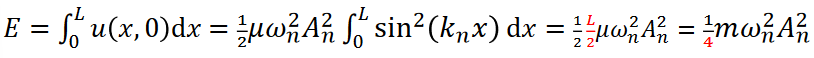
\includegraphics[width=0.65\textwidth]{screenshots/2024-03-21-09-26-14.png}
\end{figure}
Non mi piace il fatto che compaia il fattore \(\frac{1}{4}\): da dove viene? Quanto appena trovato viene dal fatto che avevamo posto \(A = -2A_i\), quindi possiamo riscrivere l'energia come
\[
	E= \frac{1}{4} m \omega _n ^{2} A_n ^{2} = m \omega _n ^{2} A_i ^{2} = \frac{1}{2} m \omega _n ^{2} A_i ^{2} + \frac{1}{2} m \omega _n^{2} A_r ^{2}
\]
\paragraph{Potenza e intensità}
La potenza trasportata dall'onda è data da:
\begin{figure}[H]
	\centering
	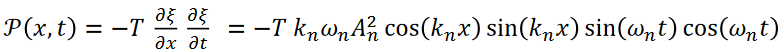
\includegraphics[width=0.65\textwidth]{screenshots/2024-03-21-09-33-30.png}
\end{figure}
Si nota immediatamente che \(\mathcal{P} (x,t) \propto \sin (2 \omega _n t)\), che ha media nulla! In questo caso \(\mathcal{P} (x,t) \neq v u(x,t)\) perché non ho un'onda progressiva. Di conseguenza non ha senso parlare di intensità, perché le onde stazionarie non trasportano energia:
\[
	I=\frac{1}{T_P}\int_{0}^{T_P} \mathcal{P} (x,t) \,\mathrm{d}t = \langle \mathcal{P} \rangle =0 \ \left(\neq \frac{1}{2}Z \omega ^{2} A ^{2} \right)
\]
\begin{exercise}
	Dimostrare che per un'onda regressiva, in cui vale \(\frac{\partial \xi }{\partial x} = \frac{1}{v} \frac{\partial \xi }{\partial t}  \), si ha \(\mathcal{P} (x,t) = T \frac{\partial \xi }{\partial x} \frac{\partial \xi }{\partial t} \).
\end{exercise}
L'esercizio sopra è il motivo per cui non ha senso parlare di intensità per le onde stazionarie: i contributi di potenza di onda progressiva e regressiva si annullano! Per convenzione decidiamo allora che la potenza sarà sempre \(\mathcal{P} (x,t) = -T \frac{\partial \xi }{\partial x} \frac{\partial \xi }{\partial t}  \) e che il suo segno avrà un significato: positivo se l'onda è progressiva, negativo se è regressiva.
\begin{exercise}
	Dimostrare che per \(\xi (x,t) = f(x-vt) + g(x+vt)\) vale \(\mathcal{P} (\xi )= Z \frac{\partial f}{\partial t} - Z \frac{\partial f}{\partial t}\).
\end{exercise}

\subsection{Approfondimento: analisi di Fourier per onde stazionarie}
Consideriamo come prima una corda vincolata in \(x=0\) e \(x=L\) (si applica l'equazione \eqref{eq:fourier_standing}):
\begin{figure}[H]
	\centering
	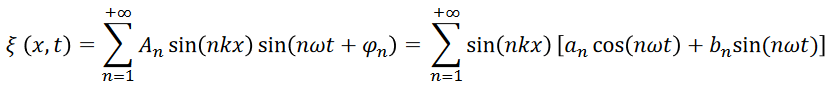
\includegraphics[width=0.65\textwidth]{screenshots/2024-03-21-09-44-56.png}
\end{figure}
Devo capire come determinare i coefficienti \(a_n\) e \(b_n\). Supponiamo di conoscere forma e velocità della corda a \(t=0\): \(\xi (x,0) = f(x),\ \dot{\xi }(x,0)=g(x)\). Impongo la condizione iniziale sulla forma (\(\sin (0)=0,\ \cos (0)=0\) quindi restano solo i coefficienti \(a_n\)):
\begin{equation}\label{eq:fourierxix0}
	\xi (x,0)= \sum_{n=1}^{\infty} a_n \sin (nkx) \equiv f(x)
\end{equation}
Le definizioni già viste di ortonormalità delle funzioni valgono anche nello spazio delle coordinate, non solo in quello dei tempi:
\begin{figure}[H]
	\centering
	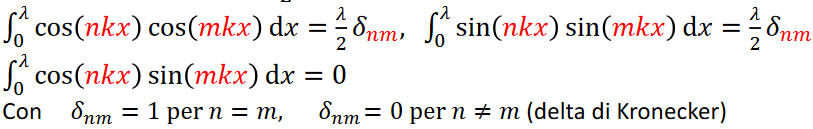
\includegraphics[width=0.65\textwidth]{screenshots/2024-03-21-09-49-54.png}
\end{figure}
Quindi \(\cos (nkx)\) e \(\sin (nkx)\) costituiscono una base ortogonale per tutte le funzioni periodiche di \(\lambda = \frac{2\pi }{k}\) nello spazio. Tuttavia nessuna delle funzioni \(\cos (nkx)\) soddisfa i vincoli (perché \(\cos (0)=1\)), abbiamo trovato una base troppo grande per rappresentare il nostro problema! Le funzioni \(\sin (nkx)\) con \(k=\pi / L\) sono una base completa in [0,L] per cui vale:
\begin{figure}[H]
	\centering
	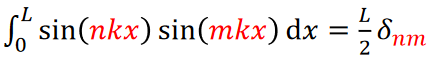
\includegraphics[width=0.5\textwidth]{screenshots/2024-03-21-09-53-31.png}
\end{figure}
Per trovare i coefficienti \(a_n\) posso moltiplicare entrambi i membri dell'equazione \eqref{eq:fourierxix0} per \(\sin (mkx)\) e integrare in [0,L]:
\begin{figure}[H]
	\centering
	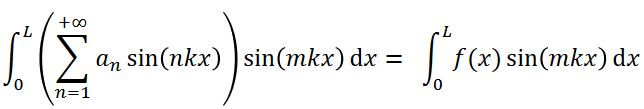
\includegraphics[width=0.65\textwidth]{screenshots/2024-03-21-09-54-27.png}
\end{figure}
Da cui si ottiene che \(a_n = \quotient{2}{L} \int_{0}^{L} f(x) \sin (nkx) \,\mathrm{d}x\) per le proprietà di ortonormalità descritte in precedenza. Dalla condizione sulla velocità si possono trovare i coefficienti \(b_n\):
\[
	\dot{\xi }(x,t) = \sum_{n=1}^{\infty} \sin (nkx)[-n \omega a_n \sin (n \omega t) + n \omega b_n \cos (n \omega t)]
\]
che al tempo 0 dev'essere
\[
	\dot{\xi }(x,0) = \sum_{n=1}^{\infty} n \omega b_n \sin (nkx) \equiv  g(x)
\]
Come prima, moltiplico per \(\sin (mkx)\) e integro in [0,L]:
\begin{figure}[H]
	\centering
	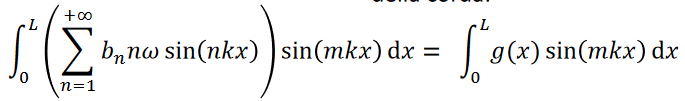
\includegraphics[width=0.65\textwidth]{screenshots/2024-03-21-09-58-29.png}
\end{figure}
Quanto appena fatto è l'equivalente di proiettare un vettore su una base, solo che è stato fatto per una funzione. Da qui, operando come prima, si giunge a 
\begin{figure}[H]
	\centering
	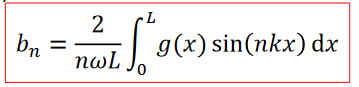
\includegraphics[width=0.45\textwidth]{screenshots/2024-03-21-09-59-51.png}
\end{figure}
In merito a quanto appena fatto c'è un bel link Desmos che rappresenta l'esercizio sulla corda pizzicata: \href{https://www.desmos.com/calculator/wd8dn38ekr}{corda pizzicata}.